\chapter{Criticality Testing}

In this chapter we describe algorithms used to determine list-criticality of graphs. Recall that we are 
not storing the explicit list assignment $L$ for our graphs, so what we want to check is whether there 
exists a $L$ so that the graph is critical with respect to that $L$. However, even if $L$ was fixed, 
it would still be a computationally hard problem to determine criticality. What we will do instead is check 
for weaker properties, and therefore admit some false positives, that is, some graphs we identify as list-critical 
for which actually no suitable $L$ exist. Our hope is that the tests will be exhaustive enough so that finiteness 
results such as \ref{linearboundcycletheorem} still hold for the weaker properties we are testing, and our algorithms 
terminate. We will see that indeed, the algorithms described here work very well in practice at discarding non-critical graphs. 

\todo{explain that we work with graphs with prescribed list sizes}

\section{Degree Properties}

We can start with an easy observation:

\begin{observation}
\label{degreeobs}
In a $f$-list-critical graph, $d(v) \geq f(v)$ for all vertices $v$.
\end{observation}

So if we find a vertex with degree less than the prescribed list size, we can conclude that the graph is not list-critical. 
However, this is a very weak test. We can incorporate another test concerning the vertices with $d(v) = |L(v)|$: there is
the following result by Gallai showing that the subgraph induced by those vertices must have a certain structure, generalizing 
the classical Brooks theorem for vertex coloring:

\begin{theorem}[Gallai \cite{gallaikritische}]
Let $G$ be a $f$-list-critical graph and let $H$ be the subgraph
of $H$ induced by the vertices with $d(v) = f(v)$. 
Then each $2$-connected component of $H$ is a complete graph or an odd cycle.
\end{theorem}

\section{Reducible Configurations}

The \emph{method of reducible configurations} is a usual technique in graph coloring problems. It consists in identifying subgraphs 
or other structures that can not appear in critical graphs. We have the following observation:

\begin{proposition}
\label{reduciblecolorableprop}
Let $G$ be an $f$-list-critical graph, and let $H$ be an induced subgraph of $G$ such that $\forall v \in H, f(v) > d_{G\setminus H}(v)$,
where $d_{G \setminus H}(v)$ is the number of neighbors of $v$ which are not in $H$. Then $H$ is not $g$-list-colorable, where $g(v) = f(v) -d_{G\setminus H}(v)$.
\end{proposition}

\begin{proof}
If $G = H$, it is immediate. Assume $H \subsetneq G$, and let $G$ be $L$-critical. 
Let $\phi$ be a coloring of $G \setminus H$, and let $L'$ be the $g$-list-assignment of $H$ given by 
$L'(v) = L(v) \setminus \{\phi(u) : u \in N_G(v), u \not\in H\}$. 
Then $H$ is not $L'$-colorable: since otherwise, the $L$-coloring $\phi$ of $G \setminus H$ would extend to $G$, contradiction.
\end{proof}

\begin{figure}
\centering
\begin{tikzpicture}[scale=0.8]
\VertexV[y=1]{A}
	\VertexV[x=-2]{B}
	\VertexV[y=-1]{C}
	\VertexV[x=2]{D}
	
	\node[above right = 2.5mm and 0.5mm of A] (A1){};
	\node[above left  = 2.5mm and 0.5mm of A] (A3){};
	
	\node[above left = 2mm and 2.5mm of B] (B1){};
	\node[left = 2.5mm of B] (B2){};
	\node[below left = 2mm and 2.5mm of B] (B3){};
	
	\node[above right = 2mm and 2.5mm of D] (D1){};
	\node[right = 2.5mm of D] (D2){};
	\node[below right = 2mm and 2.5mm of D] (D3){};
	
	\node[below right = 2mm and 2.5mm of C] (C1){};
	\node[below = 2.5mm of C] (C2){};
	\node[below left = 2mm and 2.5mm of C] (C3){};
	
	\Edge(A)(A1)
	\Edge(A)(A3)
	
	\Edge(B)(B1)
	\Edge(B)(B2)
	\Edge(B)(B3)
	
	\Edge(C)(C1)
	\Edge(C)(C2)
	\Edge(C)(C3)
	
	\Edge(D)(D1)
	\Edge(D)(D2)
	\Edge(D)(D3)
		
	\Edge(A)(B)
	\Edge(A)(C)
	\Edge(A)(D)
	\Edge(B)(C)
	\Edge(C)(D)

\end{tikzpicture}
\begin{tikzpicture}
\node[] at (0, 1.3) {$\implies$};
\node[] at (0, 0) {};
\end{tikzpicture}
\begin{tikzpicture}[scale=0.8]
\VertexIII[y=1]{A}
	\VertexII[x=-2]{B}
	\VertexII[y=-1]{C}
	\VertexII[x=2]{D}
	
		\node[above right = 2.5mm and 0.5mm of A] (A1){};
	\node[above left  = 2.5mm and 0.5mm of A] (A3){};
	
	\node[above left = 2mm and 2.5mm of B] (B1){};
	\node[left = 2.5mm of B] (B2){};
	\node[below left = 2mm and 2.5mm of B] (B3){};
	
	\node[above right = 2mm and 2.5mm of D] (D1){};
	\node[right = 2.5mm of D] (D2){};
	\node[below right = 2mm and 2.5mm of D] (D3){};
	
	\node[below right = 2mm and 2.5mm of C] (C1){};
	\node[below = 2.5mm of C] (C2){};
	\node[below left = 2mm and 2.5mm of C] (C3){};
	
	\Edge(A)(B)
	\Edge(A)(C)
	\Edge(A)(D)
	\Edge(B)(C)
	\Edge(C)(D)

\end{tikzpicture}
\caption{Illustration of \ref{reducibleobs}: from a subgraph, we get a graph with prescribed list sizes.}
\end{figure}

We can consider \ref{degreeobs} to be a particular case of \ref{reduciblecolorableprop}. 
In \ref{reduciblecolorablefigure} we see a couple of examples of small graphs that are always $f$-colorable,
so one possible test we can add to our criticality testing procedure is to search for occurrences of those graphs as induced subgraphs,
and if one is found then conclude that the graph is not critical.



\begin{figure}

\centering
\begin{subfigure}{0.4\textwidth}
\begin{tikzpicture}
\VertexIII[y=1]{A}
	\VertexII[x=-2]{B}
	\VertexII[y=-1]{C}
	\VertexII[x=2]{D}
	
		\node[above right = 2.5mm and 0.5mm of A] (A1){};
	\node[above left  = 2.5mm and 0.5mm of A] (A3){};
	
	\node[above left = 2mm and 2.5mm of B] (B1){};
	\node[left = 2.5mm of B] (B2){};
	\node[below left = 2mm and 2.5mm of B] (B3){};
	
	\node[above right = 2mm and 2.5mm of D] (D1){};
	\node[right = 2.5mm of D] (D2){};
	\node[below right = 2mm and 2.5mm of D] (D3){};
	
	\node[below right = 2mm and 2.5mm of C] (C1){};
	\node[below = 2.5mm of C] (C2){};
	\node[below left = 2mm and 2.5mm of C] (C3){};
	
	\Edge(A)(B)
	\Edge(A)(C)
	\Edge(A)(D)
	\Edge(B)(C)
	\Edge(C)(D)

\label{fig:reducible1}
\end{tikzpicture}
\end{subfigure}
\begin{subfigure}{0.4\textwidth}
\begin{tikzpicture}
\VertexIII[x=-1,y=2]{A1}
	\VertexIII[x=1,y=2]{A2}
	\VertexII[x=-2]{B1}
	\VertexII[y=-1.25]{B2}
	\VertexII[x=2]{B3}
	\VertexV[y=0.5]{C}
	
	\Edge(C)(A1)
	\Edge(C)(A2)
	\Edge(C)(B1)
	\Edge(C)(B2)
	\Edge(C)(B3)
	\Edge(A1)(A2)
	\Edge(A2)(B3)
	\Edge(B3)(B2)
	\Edge(B2)(B1)
	\Edge(B1)(A1)

\end{tikzpicture}
\label{fig:reducible2}
\end{subfigure}
\caption{Some colorable reducible configurations.}
\label{fig:colorablereducible}
\end{figure}

However, there are also reducible configurations which are not $f$-colorable.

\begin{definition}
A graph $G$ is said to be \emph{$f$-reducible} if there is a proper subgraph $H \subsetneq G$ so that
for all $f$-list-assignments $L$ of $G$, if $H$ is $L\restriction_H$-colorable then $G$ is $L$-colorable. 
\end{definition}

\begin{proposition}
Let $G$ be an $f$-list-critical graph, and let $H$ be an induced subgraph of $G$ such that $\forall v \in H, f(v) > d_{G\setminus H}(v)$,
where $d_{G \setminus H}(v)$ is the number of neighbors of $v$ which are not in $H$. Then $H$ is not $g$-reducible, where $g(v) = f(v) -d_{G\setminus H}(v)$.
\end{proposition}

\begin{proof}
Assume not, and let $H'$ be the corresponding subgraph of $H$ for which all $g$-colorings extend. Let $G$ be $L$-critical. 
There exists an $L$-coloring $\phi$ of $G \setminus (H \setminus H')$. Let $L'$ be the $g$-list-assignment of $H$ given by 
$L'(v) = L(v) \setminus \{\phi(u) : u \in N_G(v), u \not\in H\}$. Note that $\phi\restriction_{H'}$ is an $L'$-coloring of $H'$, so there must
be an $L'$-coloring $\psi$ of $H$. But then the coloring $\Phi$ given by $\Phi(v) = \psi(v)$ for $v \in H$, $\Phi(v) = \phi(v)$ for $v \in G \setminus H$ is 
a $L$-coloring of $G$, contradiction. 
\end{proof}

\begin{figure}

\centering
\begin{tikzpicture}
\VertexIV[y=1, label=$u$,position=above]{X}
	\VertexII[x=-3, y=-1, label=$v$, position=below]{A}
	\VertexII[x=-1, y=-1, label=$w$,position=below]{B}
	\VertexII[x=1, y=-1, label=$x$,position=below]{C}
	\VertexII[x=3, y=-1, label=$y$,position=below]{D}
	
	\Edge(X)(A)
	\Edge(X)(B)
	\Edge(X)(C)
	\Edge(X)(D)
	\Edge(A)(B)
	\Edge(B)(C)
	\Edge(C)(D)

\end{tikzpicture}
\caption{A non-colorable reducible configuration.}
\label{fig:noncolorablereducible}
\end{figure}

\begin{observation}
The graph depicted in \ref{fig:noncolorablereducible} with prescribed list sizes $f$ is $f$-reducible.
\end{observation}

\begin{proof}
Let us characterize the $f$-list-assignments $L$ for which the graph is not $L$-colorable. First, note that if $L(v) \neq L(w)$ or $L(x) \neq L(y)$
one can precolor both $w$ and $x$ so that the resulting graph with the corresponding colors removed from the lists is a path with list sizes at least $2$
in all vertices except in one endpoint, with list size at least $1$, so it is colorable. Therefore, we have $L(v) = L(w)$ and $L(x) = L(y)$. Then, note
that $L(v), L(x) \subseteq L(u)$, since otherwise by coloring one vertex with a color not in $L(u)$ one can always color the graph. Therefore, the $f$-list-assignments
for which the graph is not $L$-colorable are those of the form $L(u) = \{A, B, C, D\}$, $L(v) = L(w) = \{A, B\}$, $L(x) = L(y) = \{C, D\}$. But for those list assignments
the graph without edge $wx$ is also not $L$-colorable, so for any $f$-list-assignment $L$ the graph is $L$-colorable if and only if the subgraph without the edge $wx$ is
$L$-colorable.
\end{proof}

\section{The Alon-Tarsi Method}

While checking for the small reducible configurations we found in the previous section is helpful, it is not good enough, because
there are larger graphs which are always $f$-colorable but do not contain any of the reducible configurations. One could augment the
list of configurations to check by manually those graphs when they are encountered, but this is ineffective and also inefficient because
induced subgraph isomorphism testing starts being very expensive with larger subgraphs. 
We would, then, like to have a systematic method to find when graphs with prescribed list sizes $f$ are $f$-list-colorable. Alon and Tarsi
provided a useful criterion:

\begin{theorem}[Alon-Tarsi, \cite{alontarsi}]
\label{alontarsitheorem}
Let $G$ be a directed graph on vertices $v_1, \ldots, v_n$, and let $L$ be an assignment of lists to vertices of $G$ such that 
$|L(v_i)| \geq d^+(v_i)+1$ for $i = 1, \ldots, n$. If $G$ has a different number of even and odd spanning eulerian subgraphs,
then $G$ has an $L$-coloring.
\end{theorem}

\todo{Define directed graphs and d+ either here or in the introduction}.

Here \emph{even} and \emph{odd} eulerian subgraphs refer to the number of edges. We will explain the proof of this theorem here,
since it will give us insight into how to implement it in a more efficient way than enumerating all eulerian subgraphs. For the
proof we will need an algebraic result known as Combinatorial Nullstellensatz.

\begin{theorem}[Combinatorial Nullstellensatz \cite{alonnullstellensatz}]
Let $\mathbb{K}$ be a field and $p(x_1, \ldots, x_n) \in \mathbb{K}[x_1, \ldots, x_n]$ be a nonzero polynomial and let $t_1, \ldots, t_n$ be nonnegative integers such that the
 degree of $p$ is $t_1 + \ldots + t_n$ and the coefficient of $\prod_{i=1}^n x_i^{t_i}$ in $p$ is nonzero. 
 Let $S_1, \ldots, S_n$ be subsets of $\mathbb{K}$ such that $|S_i| \geq t_i+1$. Then there exist $a_1 \in S_1, \ldots, a_n \in S_n$ such that
$p(a_1, \ldots, a_n) \neq 0$.
\end{theorem}

\subsection{Proof of the Alon-Tarsi Theorem}

\begin{definition}
For a directed graph $G$ with $n$ vertices $v_1, \ldots, v_n$, we define its \emph{graph polynomial} $p_G(x_1, \ldots, x_n)$ as:
\begin{equation}
\label{eq:graphpolynomialproduct}
p_G(x_1, \ldots, x_n) = \prod_{\overrightarrow{v_iv_j}\in E(G)} (x_j-x_i).
\end{equation}
\end{definition}


\begin{observation}
If we associate each color with a different number (we work in, say, $\mathbb{C}$), then $\phi$ is a proper coloring of 
$G$ if and only if $p_G(\phi(v_1), \ldots, \phi(v_n)) \neq 0$. 
\end{observation}

\begin{proposition}
\ref{polynomialatproposition}
Let $G$ be as in the hypothesis of the Alon-Tarsi theorem.
If the coefficient of $p_G$ at $\prod_{i=1}^n x_i^{d^+(v_i)}$ is non-zero, then $G$ has an $L$-coloring.
\end{proposition}
\begin{proof}
The total degree of $p_G$ is $|E(G)| = d^+(v_1) + \ldots + d^+(v_n)$. By the Combinatorial Nullstellensatz, 
one can find $\phi(v_1) \in L(v_1), \ldots, \phi(v_n) \in L(v_n)$ so that $p_G(\phi(v_1), \ldots, \phi(v_n)) \neq 0$.
\end{proof}

\begin{observation}
Let $G$ be a directed graph, and denote by $x_G = \prod_{\overrightarrow{v_iv_j} \in E(G)} x_j$. Let $D_1$ and $D_2$ be two orientations of a graph, denote by
$|D_1 \Delta D_2|$ the number of edges with different direction in the two orientations. We have:
\begin{equation}
\label{eq:graphpolynomialsum}
p_G(x_1, \ldots, x_n) = \sum_{D \text{ orientation of } G} (-1)^{|D\Delta G|} x_D
\end{equation}
\end{observation}

\begin{proposition}
\label{proplastalontarsi}
The absolute value of the coefficient of $p_G$ at $\prod_{i=1}^n x_i^{d^+(v_i)}$ is the difference between odd and even eulerian spanning subgraphs of $G$.
\end{proposition}

\begin{proof}
Consider the set $\mathcal{S} = \{D \text{ orientation of } G : x_D = \prod_{i=1}^n x_i^{d^+(v_i)} \}$, that is, 
the set of orientations which have the same indegrees as $G$. We claim that this set is in bijection 
with the set of eulerian spanning subgraphs of $G$, with a bijection maps orientations with even 
$|D\Delta G|$ to even spanning subgraphs and orientations with odd $|D\Delta G|$ to odd spanning
subgraphs. This implies the result by \eqref{eq:graphpolynomialsum}.

The bijection is as follows: for each $D \in \mathcal{S}$ map it to the subgraph with edges given by 
the edges in $G$ which have opposite orientation as edges in $D$. Since the indegrees of $D$ and $G$ are 
the same, this subgraph is eulerian, and this map is clearly invertible and hence a bijection. 
\end{proof}

This concludes the proof of \ref{alontarsitheorem}.

\subsection{Implementation of the Alon-Tarsi Method}

Here we will explain how to use \ref{alontarsitheorem} in practice to check the $f$-colorability of a graph.  The first thing we have to note
is that \ref{alontarsitheorem} is stated with respect to a directed graph, but this is immaterial to our needs. We only have the prescribed
list sizes $f$, and for each such prescription there can be different orientations of that satisfy the $f(v) \geq d^+(v) + 1$ condition, 
and we could apply the theorem to each of those. So instead of using the combinatorial characterization of \ref{alontarsitheorem}, what we will
do is directly compute the polynomial $p_G$ with respect to an arbitrary orientation of the graph, and if any monomial $\prod x_i^{e_i}$ with 
$e_i < f(i)$ has a nonzero coefficient we will conclude $f$-colorability. 

It will be convenient to think of the computation of the polynomial $p_G$ using the expression \eqref{eq:graphpolynomialsum}. This way, we can compute the 
coefficients by enumerating all orientations of the graph and summing the signs.  The implementation is as follows:

\begin{algorithm}
\caption{Naive Alon-Tarsi.}
\SetAlgoLined
\SetKwComment{Comment}{/* }{ */}
\SetKwProg{Fn}{function}{}{end}
\Comment*[r]{Returns true if the Alon-Tarsi method determines that $G$ is $f$-colorable.}
\Fn{alonTarsi($G$, $f$)}{
	$S \gets \text{allOrientations(G)}$\; 
	\Comment*[r]{allOrientations($G$) generates all orientations of $G$ (e. g. by orienting each edge by recursive backtracking)}
	$p_G \gets \text{emptyAssociativeArray()}$\; 
	\Comment*[r]{We represent the polynomial $p_G$ by an associative array mapping the array of
	 $n$ integers $e_1, \ldots, e_n$ to the coefficient of $\prod x_{i}^{e_{i}}$ initialized to $0$ on all values.}
	\For{$D \in S$}{
		$s \gets 1$\;
		$e \gets \text{array}(n)$\;
		\For{$\{u, v\} \in E(G)$} {
			\Comment*[r]{We pick an arbitrary order for $u, v$ in each edge in order to determine an arbitrary orientation of $G$
			(e. g. set $u < v$ in the integer labeling we use to represent $G$).}
			\uIf{$\overrightarrow{uv} \in E(D)$} {
				$e_v \gets e_v + 1$\;
			}
			\uElse{
				$s \gets -s$\;
				$e_u \gets e_u + 1$\;
			}
		}
		$p_G[e] \gets p_G[e] + s$\;
	}
	\For{$(e, c_e) \in p_G$} {
		\Comment*[r]{Iterate over the coefficients of the polynomial and if there is some nonzero coefficient of an appropiate monomial, return success.}
		\If{$e_v < f(v) \, \forall v \in V(G)$ } {
			\If{$c_e \neq 0$} {
				return true\;
			}
		}
	}
	return false\; 
	
}
\end{algorithm}

However, there are multiple improvements that can be made over this naive implementation.

The most immediate one is that we only care about the coefficients of the monomials
corresponding to orientations with indegrees less than $f(v)$ in each vertex $f$ 
(we call such orientations \emph{$f$-bounded orientations}, and the coefficients of the 
corresponding terms of the polynomial
\emph{$f$-bounded coefficients}).
Therefore we can store only coefficients of the polynomial corresponding to $f$-bounded orientations.
We would also like to generate only $f$-bounded orientations, so that we do not have to iterate over all 
$2^|E(G)|$ orientations of the graphs. 

If we generate orientations by a orienting each edge one by
one in a recursive backtracking fashion, we want to know when to cut a branch that is not going to lead
to an $f$-bounded orientation. The easiest way is to cut a branch when the 
branch trivially does not correspond
anymore to an $f$-bounded orientation, that is, 
when the indegree of some of the vertices already reaches $f(v)$. 
It can be done in a more sophisticated way by reducing the problem of checking whether a partial 
orientation can be extended to an $f$-bounded 
orientation to a problem of maximum bipartite matching. This way,
all the branches that do not lead to an $f$-bounded 
orientation can be immediately discarded by this test, and 
we can obtain an enumeration of all $f$-bounded orientations in polynomial time for each 
$f$-bounded orientation.

However, it turns out it is more efficient to just do it in the trivial way since the overhead of solving
the bipartite matching subproblems is not worth the more eager cutting of branches. The trivial branch cutting
can be improved by selecting the next edge that is going to be oriented following some heuristic
that makes it more likely for branches to be cut off earlier. 
For example, we can orient first the edges that whose orientation is forced 
(because one of the endpoints has already indegree $f(v)-1$) 
and then prioritize the ones whose both endpoints have indegrees close to $f(v)$.

Implementing the above improvements already makes a very substantial impact in the execution time
of the algorithm, but it is still slow when the number of $f$-bounded orientations is very large
and storing all the $f$-bounded coefficients of the polynomial can also incur in a large memory usage.

There is a different approach which can work a bit better in practice, based not on enumerating
all orientations but on computing the contribution of each edge to the polynomial separately. 
We can think of it as using \eqref{eq:graphpolynomialproduct} instead of \eqref{eq:graphpolynomialsum} and
computing the product $\prod_{\overrightarrow{v_iv_j} \in E(G)} (x_i - x_j)$ term by term.
The important ideas in making this be actually faster than the enumerating orientations approach are:

\begin{itemize}
	\item We \emph{truncate} the partial results so that we don't store non-$f$-bounded coefficients:
	we only care about $f$-bounded coefficients, so we can just avoid storing the other coefficients of the 
	polynomial, not only in the final result but also in the intermediate results we get after multiplying each
	$(x_i-x_j)$ term. 
	
	In a similar fashion to the previous discussion in which we were enumerating $f$-bounded orientations, given 
	the intermediate polynomial after multiplying some of the terms we can check whether each monomial will have
	some contribution to a $f$-bounded coefficient in the final result - i.e., whether the partial orientations
	corresponding to the indegree sequence corresponding to the monomial can be extended to a $f$-bounded orientations
	- by solving a bipartite matching problem. But, just as before, we find that the overhead of performing this
	extendability test is not worth the additional pruning and that it is more efficient in practice to just discard
	non-$f$-bounded monomials. 
	
	
	\item We also discard monomials whose coefficients are $0$ in the intermediate results and don't store them in
	memory. This is the most important optimization and it is what makes this approach better in practice than the
	one about enumerating orientations, since in ``hard-to-color'' graphs we expect that we will already start seeing
	many zeroes in intermediate results and this can contribute to an important reduction in time and memory usage.
	
	\item As before, the order in which we process edges matters. We want to have many truncations and 
	zero coefficents early, so that we store data for our partial results. This can be done heuristically 
	by prioritizing edges with small values of $f$ at their endpoints. 

\end{itemize}


\begin{algorithm}
\caption{Optimized Alon-Tarsi with truncated multiplication.}
\SetAlgoLined
\SetKwComment{Comment}{/* }{ */}
\SetKwProg{Fn}{function}{}{end}
\Comment*[r]{Returns true if the Alon-Tarsi method determines that $G$ is $f$-colorable.}
\Fn{alonTarsi($G$, $f$)}{
	
	$p_G \gets \text{emptyAssociativeArray()}$\; 
	$E \gets \text{sortEdges}(E(G), f)$\;
	\Comment*[r]{sortEdges sorts the edges according to some heuristic, e.g. increasing by sum of values of $f$ at endpoints}
	\For{$\{u, v\} \in E$}{
		$q \gets \text{emptyAssociativeArray()}$\; 
		\Comment*[r]{$q = p_G (x_u - x_v)$}
		
		\For{$(e, c_e) \in p_G$} {
			\If{$e_u+1 < f(u)$} {
				$r \gets e$\;
				$r_u \gets r_u+1$\;
				$q[r] \gets q[r] + c_e$\;
			}
			\If{$e_v+1 < f(v)$} {
				$r \gets e$\;
				$r_v \gets r_v+1$\;
				$q[r] \gets q[r] - c_e$\;
			}
		}
		$p_G \gets \text{emptyAssociativeArray()}$\; 
		\Comment*[r]{Update $p_G$ with the nonzero coefficients of $q$}.
		\For{$(e, c_e) \in q_G$} {
			\If{$c_e \neq 0$} {
				$p_G[e] \gets c_e$\;
			}
		}
	
	}
	\For{$(e, c_e) \in p_G$} {
		\If{$c_e \neq 0$} {
			return true\;
		}
		
	}
	return false\; 
	
}


\end{algorithm}

Further improvements are possible, but we do not describe them here since this is already the implementation we have actually used for this project. 
For a more detailed analysis and comparison of techniques for the efficient implementation 
of the Alon-Tarsi method, see \cite{dvorakefficientalontarsi}.


Remember that the Alon-Tarsi method does not always detect colorable graphs successfully. 
For example, the graph in \ref{fig:reducible2} is not recognized by Alon-Tarsi as a colorable graph. \todo{fix reference to reducible configuration figure}
In addition, for bigger graphs Alon-Tarsi is significantly slower than the search for fixed small induced subgraphs.
So it is still advisable to first check for the small 
reducible configurations we found above before running Alon-Tarsi. 

\section{Recursive Colorability Testing}

We know that if our graph has a reducible configuration as an induced subgraph, then it can not
be $f$-critical. And we can determine whether a induced subgraph is an always-colorable reducible 
configuration using the Alon-Tarsi method. So one possible idea would be to apply Alon-Tarsi on 
every induced subgraph to check if our graph has any reducible configuration. We can easily see 
that this is not very efficient - we run the already slow Alon-Tarsi method on an exponential 
number of graphs. On the other extreme, we can run the Alon-Tarsi method only on the entire 
graph, falsifying $f$-criticality only if it is $f$-colorable. This is not good, either - we can 
easily imagine graphs which are not $f$-colorable but are not $f$-critical either, 
because they contain some reducible configuration as an induced subgraph. 


\begin{figure}
\label{fig:recursivereducibility}
\centering
\begin{subfigure}{0.4\textwidth}
\begin{tikzpicture}[scale=0.6]
\VertexV[y=-1]{A}
	\VertexV[x=-2]{B}
	\VertexV[y=1]{C}
	\VertexV[x=2]{D}
	
	\VertexV[x=-2,y=-2]{E}
	\VertexV[x=2,y=-2]{F}
	\VertexV[y=-3.5]{G}
	
	\VertexI[x=-1.5,y=2]{V1}
	\VertexI[x=0,y=2]{V2}
	\VertexI[x=1.5,y=2]{V3}
	
	\VertexI[x=3.75,y=-1.5]{V4}
	\VertexI[x=3.5,y=-2.25]{V5}
	
	\VertexI[x=-1,y=-5]{V8}
	\VertexI[x=0,y=-5]{V7}
	\VertexI[x=1,y=-5]{V6}
	
	\VertexI[x=-3.75,y=-1.5]{V10}
	\VertexI[x=-3.5,y=-2.25]{V9}
	
	
	\Edge(A)(B)
	\Edge(A)(C)
	\Edge(A)(D)
	\Edge(B)(C)
	\Edge(C)(D)
	
	\Edge(E)(F)
	\Edge(F)(G)
	\Edge(G)(E)
	
	\Edge(E)(A)
	\Edge(F)(A)	
	\Edge(E)(B)
	\Edge(F)(D)
	
	
	\Edge(V1)(V2)
	\Edge(V2)(V3)
	\Edge(V3)(V4)
	\Edge(V4)(V5)
	\Edge(V5)(V6)
	\Edge(V6)(V7)
	\Edge(V7)(V8)
	\Edge(V8)(V9)
	\Edge(V9)(V10)
	\Edge(V10)(V1)
	
	\Edge(V1)(C)
	\Edge(V1)(B)
	\Edge(V2)(C)
	\Edge(V3)(C)
	\Edge(V3)(D)
	\Edge(V4)(D)
	\Edge(V4)(F)
	\Edge(V5)(F)
	\Edge(V6)(F)
	\Edge(V6)(G)
	\Edge(V7)(G)
	\Edge(V7)(G)
	\Edge(V8)(G)
	\Edge(V8)(E)
	\Edge(V9)(E)
	\Edge(V10)(E)
	\Edge(V10)(B)

\end{tikzpicture}
\end{subfigure}
\begin{subfigure}{0.1\textwidth}
\begin{tikzpicture}
\node[] at (0, 0) {$\implies$};
%\node[] at (0, 0) {};
\end{tikzpicture}
\end{subfigure}
\begin{subfigure}{0.4\textwidth}
\begin{tikzpicture}[scale=0.6, yshift=5cm]
\VertexV[y=-1]{A}
	\VertexIII[x=-2]{B}
	\VertexII[y=1]{C}
	\VertexIII[x=2]{D}
	
	\VertexII[x=-2,y=-2]{E}
	\VertexII[x=2,y=-2]{F}
	\VertexII[y=-3.5]{G}
	
	
	
	\Edge(A)(B)
	\Edge(A)(C)
	\Edge(A)(D)
	\Edge(B)(C)
	\Edge(C)(D)
	
	\Edge(E)(F)
	\Edge(F)(G)
	\Edge(G)(E)
	
	\Edge(E)(A)
	\Edge(F)(A)	
	\Edge(E)(B)
	\Edge(F)(D)

\end{tikzpicture}
\end{subfigure}
\caption{An example of a non-$f$-colorable graph with a reducible configuration obtained from a cycle-canvas.}
\end{figure}

In fact, as \ref{fig:recursivereducibility} shows, this scenario can happen very easily when, 
for example, generating critical cycle-canvases, because it suffices to have a triangle with list 
sizes $2$ to make the graph non-$f$-colorable. The specific reducible configuration that appears 
in \ref{fig:recursivereducibility} is one of the small ones that we can check specifically before 
running Alon-Tarsi, but the more general scenario of having a reducible configuration plus a 
non-colorable subgraph does also often happen with larger reducible configurations and it is 
important that we deal with it automatically, using Alon-Tarsi to detect the reducible 
configuration.

What we do is the following: if Alon-Tarsi returns a negative answer to being applied to the 
entire graph, we try to find a \emph{minimal} non-colorable subgraph which is causing this 
negative answer (such 
as the triangle in \ref{fig:recursivereducibility}). We do that by arbitrarily removing vertices
and checking whether the graph is still non-$f$-colorable, and doing so until we have a graph
which becomes $f$-colorable when any vertex is removed. Then we remove subgraph $H$ (and reduce
the list sizes of vertices neighboring $H$ correspondingly, like when considering reducible 
configurations) and recursively apply the test to the remaining graph. We see that this works for
the graph in \ref{fig:recursivereducibility}: first, the triangle is removed and then the 
reducible configuration is identified. This recursive approach also handles more general cases
when there are multiple non-colorable subgraphs obstructing the colorability of the entire graphs.
Overall, the results of using this heuristic are very satisfactory. 

\begin{algorithm}[H]
\caption{Recursive Colorability Testing.}
\SetAlgoLined
\SetKwProg{Fn}{function}{}{end}
\SetKwComment{Comment}{/* }{ */}
\Fn{containsColorableSubgraph(G)}{
\If{$G$ is empty} {
	return false\;
}
\If{alonTarsi($G$)} {
	return true\;
}
$H \gets \text{minimalNonColorable}(G)$\;
return containsColorableSubgraph($\text{precolorSubgraph}(G,H)$)\;
\Comment*[r]{$\text{precolorSubgraph}(G,H)$ returns the graph $G$ removing the subgraph $H$ and decrementing the list sizes of the neighbors of vertices of $H$ appropiately.}
}
\Fn{minimalNonColorable(G)}{
	\For{$v \in V(G)$} {
		\If{not alonTarsi(removeVertex($G$,$v$))} {
			return minimalNonColorable(removeVertex($G$,$v$))\;
		}
	}
	return $G$\;
}


\end{algorithm}
\section{Criticality Verification}

\todo{Determine whether Criticality Verification section should be written and do so if necessary}
